\documentclass[reqno]{amsart}

\usepackage{amsfonts,latexsym,amsthm,amssymb,amsmath,amscd,euscript,bm}
\usepackage[sc]{mathpazo}
\usepackage[margin = 2cm]{geometry}
\usepackage{enumitem}
\usepackage{hyperref}
% sets numbering of enumerate to a, b, c, ...
\renewcommand{\theenumi}{\alph{enumi}}

% Theorems, propositions, etc.
\newtheorem{theorem}{Theorem}
\newtheorem{proposition}[theorem]{Proposition}
\newtheorem{lemma}[theorem]{Lemma}
\newtheorem{corollary}[theorem]{Corollary}

\theoremstyle{definition}
\newtheorem{definition}[theorem]{Definition}
\newtheorem*{claim}{Claim}

\theoremstyle{remark}
\newtheorem*{remark}{Remark}
\newtheorem*{notation}{Notation}
\newtheorem*{example}{Example}
\usepackage{tikz-cd}


% Math blackboard font
\newcommand{\nc}{\newcommand}
\nc{\on}[1]{\operatorname{#1}}

\nc{\R}{\mathbb R}
\nc{\C}{\mathbb C}
\nc{\Q}{\mathbb Q}
\nc{\Z}{\mathbb Z}
\nc{\N}{\mathbb N}
\nc{\HH}{\mathbb H}
\nc{\DD}{\mathbb D}
\nc{\TT}{\mathbb T}
\nc{\EE}{\mathbb E}
\nc{\FF}{\mathbb F}

\nc{\cT}{\mathcal T}
\nc{\cA}{\mathcal A}
\nc{\cM}{\mathcal M}
\nc{\cR}{\mathcal R}
\nc{\cB}{\mathcal B}
\nc{\cG}{\mathcal G}
\nc{\cD}{\mathcal D}
\nc{\cS}{\mathcal S}
\nc{\cF}{\mathcal F}
\nc{\cL}{\mathcal L}
\nc{\cE}{\mathcal E}

\nc{\GL}{\mathsf{GL}}
\nc{\Unit}{\mathsf U}
\nc{\Orth}{\mathsf O}
\nc{\Fr}{\operatorname{Fr}}

\nc{\im}{\operatorname{im}}

\nc{\diam}{\operatorname{diam}}
\nc{\supp}{\operatorname{supp}}



% Why the f*** would you ever use \epsilon
\renewcommand{\epsilon}{\varepsilon}
\renewcommand{\emph}{\textsc}
\renewcommand{\Re}{\operatorname{Re}}
\renewcommand{\Im}{\operatorname{Im}}


\let\vec\textbf

% Title: change problem set number as needed
\title
{
	\emph{Differential forms}
} 

\author{Jason Zhao}
\date{\today}

\begin{document}
\maketitle
\tableofcontents

\section{Linear algebra}

Let $V$ be an $n$-dimensional real vector space, and denote $V^*$ its dual space. Given a basis $\{e_i\}_i$, there exists a dual basis $\{\epsilon^j\}_j \subseteq V^*$ satisfying 
	\[ \langle e_i, \epsilon^j \rangle = \delta^j_i. \]
Choose another basis $\{\widetilde e_i\}_i \subseteq V$ and denote its dual basis by $\{\widetilde \epsilon^j\}_j \subseteq V^*$. There exists a change of basis matrix $L^k_i \in \mathsf{GL} (\R^n)$ sending the original basis to the new basis,
	\[ \widetilde e_i = L^k_i e_k. \]	
On the other hand, the inverse change of basis matrix $(L^{-1})^j_k \in \mathsf{GL} (\R^n)$, i.e. $(L^{-1})^j_k L^k_i = \delta^j_i$, transforms the original dual basis to the new dual basis 	
	\[ \widetilde \epsilon^j = (L^{-1})^j_k \epsilon^k. \]

\paragraph*{\textbf{Contravariance}}

We say an object is \emph{contravariant} if the coordinate representation transforms by the inverse matrix $(L^{-1})^j_i$ when changing basis. Such coordinates are indexed by \textit{upper indices}. The prototypical example of a contravariant object is a \emph{vector} $v \in V$. Every vector admits a unique coordinate representation $\{v^i\}_i \subseteq \R$ with respect to the basis $\{e_i\}_i$, i.e.
	\[ v = v^i e_i . \]
Let $\{ \widetilde v^j \}_j \subseteq \R$ be the unique coordinates with respect to the basis $\{\widetilde e_j\}_j$, then the change of coordinates from $\{v^i\}_i$ to $\{\widetilde v^j\}_j$ is given by the inverse change of basis matrix,
	\[ \widetilde v^j = {(L^{-1})}^j_i v^i. \]
Indeed, 	
	\[ v = \widetilde v^j \widetilde e_j  = \left( {(L^{-1})}^j_i v^i \right) \left( L^k_j e_k \right) = \delta^k_i v^i e_k = v^i e_i . \]
We can interpret a choice of basis $\{e_i\}_i$ as endowing $V$ with a ``measuring tool'', where the coordinates $\{v^i\}_i$ representing the resulting ``measurement''. A change of basis corresponds to changing the choice of ``measuring tool'', e.g. we can view a change of basis $\widetilde e_i = \tfrac{1}{100} e_i$ as changing from ``meters'' $e_i$ to ``centimeters'' $\widetilde e_i$, so the corresponding change of coordinates is 
	\[ \widetilde v^i \text{ meters } = 100 v^i \text{ centimeters}. \]




\paragraph*{\textbf{Covariance}}

We say that an object is \emph{covariant} if the coordinate representation transforms by the matrix $L^k_i$ when changing basis. Such coordinates are indexed by \textit{lower indices}. The prototypical example of a covariant object is a \emph{covector} $\omega \in V^*$. Every covector admits a unique coordinate representation $\{\omega_i \}_i \subseteq \R$ with respect to the basis $\{\epsilon^i\}_i$, i.e.
	\[ \omega = \omega_i \epsilon^i = \widetilde \omega_j \widetilde \epsilon^j. \]
Let $\{\widetilde \omega_j \}_j \subseteq \R$ be the unique coordinates with respect to the basis $\{\widetilde \epsilon^j\}_j$, then the change of coordinates from $\{\omega_i\}_i$ to $\{\widetilde \omega_j\}_j$ is given by the change of basis matrix,
	\[ \widetilde \omega_j = L^i_j \omega_i \]
Indeed, 
	\[ \omega = \widetilde \omega_j \widetilde \epsilon^j = \left( L^i_j \omega_i \right) \left( (L^{-1})_k^j \epsilon^k \right) =  \delta^i_k \omega_i \epsilon^k = \omega_i \epsilon^i. \]
Scalars are regarded as ``dimensionless'' quantities, so since a covector acting on a vector produces a scalar, they have inverse dimensions. For example, we can view a change of basis $\widetilde \epsilon^j = 100 \epsilon^j$ as changing from  ``meters$^{-1}$'' $\epsilon^j$ to ``centimeters$^{-1}$'' $\widetilde \epsilon^j$, so the corresponding change of coordinates is 
	\[ \widetilde \omega_j \text{ meters$^{-1}$} = \frac{1}{100} \omega_j  \text{ centimeters$^{-1}$}. \]


	
	

\section{Tensor algebra}



\paragraph*{\textbf{Multi-linear definition}}

A \emph{$(k, \ell)$-tensor} is a $(k + \ell)$-linear functional
	\[ \overbrace{V^* \times \dots \times V^*}^{\text{$k$-copies}} \times \overbrace{V \times \dots \times V}^{\text{$\ell$-copies}}  \to \R. \]
We denote the space of $(k, \ell)$-tensors by $T^{(k, \ell)} (V)$; by convention $T^{(0, 0)} (V) := \R$. More precisely, this is the space of tensors which are $k$-contravariant and $\ell$-covariant. There exists an associative and commutative operation known as the \emph{tensor product} $\otimes : T^{(k, \ell)}(V) \times T^{(p, q)}(V) \to T^{(k + p, \ell + q)}(V)$ defined by 
	\[ (F \otimes G) (\omega^1, \dots, \omega^{k + p}, v_1, \dots, v_{\ell + q}) = F(\omega^1, \dots, \omega^k, v_1, \dots, v_\ell) G(\omega^{k + 1}, \dots, \omega^{k + p}, v_{\ell + 1} + v_{\ell + q}). \]

\paragraph*{\textbf{Coordinate definition}}

The tensor products of the basis vectors $\{ e_{i_1} \otimes \dots \otimes e_{i_k} \otimes \epsilon^{j_1} \otimes \dots \otimes \epsilon^{j_\ell} \}_{I, J} \subseteq T^{(k, \ell)} (V)$ forms a basis for the space of $(k, \ell)$-tensors. Thus every tensor admits a unique coordinate representation $\{ T^{i_1\dots i_k}_{j_1 \dots j_\ell} \}_{I, J} \subseteq \R$ with respect to the basis $\{ e_i \}_i$, i.e.
	\[ T = T^{i_1\dots i_k}_{j_1 \dots j_\ell} e_{i_1} \otimes \dots \otimes e_{i_k} \otimes \epsilon^{j_1} \otimes \dots \otimes \epsilon^{j_\ell}. \]
Let $\{ \widetilde T^{i_1'\dots i_k'}_{j_1' \dots j_\ell'} \}_{I, J} \subseteq \R$ be the unique coordinates with respect to the basis $\{\widetilde e_j\}_j$, then to change coordinates from $\{ T^{i_1\dots i_k}_{j_1 \dots j_\ell} \}_{I, J}$ to $\{ \widetilde T^{i_1'\dots i_k'}_{j_1' \dots j_\ell'} \}_{I, J}$, the upper indices transform contravariantly, i.e. with respect to the inverse change of basis matrix, and the lower indices transform covariantly, i.e. with respect to the change of basis matrix, 
	\[ \widetilde T^{i_1'\dots i_k'}_{j_1' \dots j_\ell'} = (L^{-1})^{i_1'}_{i_1} \cdots  (L^{-1})^{i_k'}_{i_k} T^{i_1\dots i_k}_{j_1\dots j_\ell} L^{j_1}_{j_1'} \cdots L^{j_\ell}_{j_\ell'}. \]
In view of the existence and uniqueness of coordinates, we can alternatively characterise a tensor as a map sending a basis for $V$ to a $(k + \ell)$-dimensional array of coordinates satisfying the transformation law above when changing bases. 
	
\vspace{1em}
\paragraph*{\textbf{Intrinsic definition}}

The prior two definitions constructed tensors and defined the space of tensors as the collection of the aforementioned constructions. To view tensors intrinsically, we first construct the space of tensors and define tensors as elements of this construction. For notational convenience, we construct the space in full generality: let $V_1, \cdots, V_k$ be real vector spaces, the \emph{free vector space} $F(V_1 \times \dots \times V_k)$ is the set of all formal linear combinations of symbols $(v_1, \dots, v_k) \in V_1 \times \dots \times V_k$. Let $R(V_1 \times \dots \times V_k) \hookrightarrow F(V_1 \times \dots \times V_k)$ be the subspace generated by the $k$-linear relations
	\[		(v_1, \dots, av_i, \dots, v_k) - a(v_1, \dots, v_i, \dots, v_k), \]
	\[	
		(v_1, \dots, v_i + w_i, \dots, v_k) - (v_1, \dots, v_i, \dots, v_k) - (v_1, \dots, w_i, \dots, v_k)
	\]
for $v_j, w_j \in W_j$ and $a \in \FF$ and $i = 1, \dots, k$. The \emph{tensor product} of $V_1, \dots, V_k$ is defined as the quotient space
	\[ V_1 \otimes \dots \otimes V_k := F(V_1 \times \dots \times V_k) / R(V_1 \times \dots \times V_k)\]
of which we denote elements via the natural projection map $F(V_1 \times \dots \times V_k) \to V_1 \otimes \dots \otimes V_k$ induced by 
	\[ (v_1, \dots, v_k) \mapsto v_1 \otimes \dots \otimes v_k. \]
It follows from definition that the tensor product of $v_1, \dots, v_k$ is $k$-linear,
\begin{align*}
	v_1 \otimes \dots \otimes a v_i \otimes \dots \otimes v_k 
		&= a(v_1 \otimes \dots \otimes v_i \otimes \dots \otimes v_k), \\
	v_1 \otimes \dots \otimes (v_i + w_i) \otimes \dots \otimes v_k
		&= v_1 \otimes \dots \otimes v_i \otimes \dots \otimes v_k + v_1 \otimes \dots \otimes w_i \otimes \dots \otimes v_k. 	
\end{align*}


\begin{theorem}[Universal property of tensor products]
	Let $V_1, \dots, V_k$ and $U$ be finite dimensional vector spaces and denote by $\iota : V_1 \times \dots \times V_k \to V_1 \otimes \dots \otimes V_k$ the $k$-linear map $(v_1, \dots, v_k) \mapsto v_1 \otimes \dots \otimes v_k$. Then for every $k$-linear map $\phi : V_1 \times \dots \times V_k \to U$, there exists a unique linear map $\widetilde \phi :  V_1 \otimes \dots \otimes V_k  \to U$ such that the diagram commutes
	\begin{center}
		\begin{tikzcd}
V_1 \times \dots \times V_k \arrow[r, "\iota"] \arrow[rd, "\phi"'] &  V_1 \otimes \dots \otimes V_k  \arrow[d, "\widetilde \phi"] \\
                                           & U                                         
\end{tikzcd}
	\end{center}
\end{theorem}

\begin{proof}
	By the universal property of free vector spaces, there exists a unique linear map $\overline \phi : F(V_1 \times \dots V_k) \to U$ induced by 
		\[ \overline \phi (v_1, \dots, v_k) := \phi(v_1, \dots, v_k).  \]
	We see from $k$-linearity of $\phi$ that $R(V_1 \times \dots \times V_k) \hookrightarrow \ker \overline \phi$, so $\overline \phi$ descends to $\widetilde \phi : V_1 \otimes \dots \otimes V_k \to U$ the unique linear map satisfying 
		\[ \widetilde \phi (v_1 \otimes \dots \otimes v_k) = \overline \phi (v_1, \dots, v_k) = \phi(v_1, \dots, v_k). \]
	The condition above can be rewritten as $\widetilde \phi \circ \iota = \phi$, completing the proof. 
\end{proof}


	\[ {(V^*)}^{\otimes k} \otimes {V}^{\otimes \ell} \cong T^{(k, \ell)} (V).  \]





	Associativity allows us to form the \emph{tensor algebra} of a finite dimensional real vector space $V$, a graded real algebra defined by 
	\[ T(V) := \R \oplus \bigoplus_{k \in \N} V^{\otimes k} \]
	where multiplication $\otimes : T(V) \times T(V) \to T(V)$ is induced by the tensor product
		\[ (v_1 \otimes \dots \otimes v_k) \otimes (v_{k + 1} \otimes \dots \otimes v_n) = v_1 \otimes \dots \otimes v_n. \]

\section{Exterior algebra}

\paragraph*{\textbf{Multi-linear definition}}

We say that a covariant $k$-tensor  $T: V^* \times \dots \times V^* \to \R$ is \emph{alternating} if its value changes sign whenever two different arguments are interchanged. More generally, 
	\[ T(\omega^1, \dots, \omega^k) = (-1)^\sigma T(\omega^{\sigma(1)}, \dots, \omega^{\sigma(k)}),\]
where $\sigma \in S_k$ is a permutation on the indices $\{1, \dots, k\}$. We denote the space of alternating covariant $k$-tensors by $\bigwedge^k V^*$. There exists an associative operation and anti-commutative operation known as the \emph{exterior product} $\wedge : \bigwedge^k V^* \times \bigwedge^\ell V^* \to \bigwedge^{k + \ell} V^*$ defined by 
	\[ (F \wedge G)(v_1, \dots, v_{k + \ell}) := \frac{1}{k! \ell!} \sum_{\sigma \in S_k} (-1)^\sigma F(v_{\sigma(1)}, \dots, v_{\sigma(k)}) G(v_{\sigma( k + 1)} ,\dots, v_{\sigma(k + \ell)}). \]

\paragraph*{\textbf{Coordinate definition}}

The wedge product of the basis vectors $\{ \epsilon^{i_1} \wedge \dots \wedge \epsilon^{i_k} \}_I \subseteq \bigwedge^k V^*$, where the indices $(i_1, \dots, i_k)$ range over strictly increasing multi-indices, forms a basis for the space of alternating covariant $k$-tensors. Thus 
	\[ \dim \bigwedge^k V^* = \binom{n}{k}, \]
where by convention the binomial coefficient is zero for $k > n$. 
	\[ T = T_{i_1 \dots i_k} \epsilon^{i_1} \wedge \dots \wedge \epsilon^{i_k}\]


\paragraph*{\textbf{Intrinsic definition}}


The \emph{exterior algebra} of a finite dimensional real vector space $V$ is the quotient graded real algebra defined by 
	\[ \bigwedge V := T(V) / I \]
where $I \subseteq T(V)$ is the $2$-sided ideal generated by elements of the form $v \otimes v$ for $v \in V$. By definition, the multiplication operation $\wedge : \bigwedge V \times \bigwedge V \to \bigwedge V$, known as the \emph{exterior product}, is induced by 
		\[ (v_1 \wedge \dots \wedge v_k) \wedge (v_{k + 1} \wedge \dots \wedge v_n) = v_1 \wedge \dots \wedge v_n. \]
and satisfies
\begin{enumerate}
	\item $k$-linearity of $(v_1, \dots, v_k) \mapsto v_1 \wedge \dots \wedge v_k$,
	\item alternating, $v \wedge v = 0$, 
	\item anti-commutative, $v \wedge w = -  (w \wedge v)$.
\end{enumerate}
We denote $\bigwedge^k V$ the space of degree $k$ terms of the exterior algebra, that is, linear combinations of terms of the form $v_1 \wedge \dots \wedge v_k$ where $v_j \in V_j$. Geometrically, degree $k$ terms capture a notion of ``oriented $k$-volume'' of the $k$-parallelopiped spanned by $v_1, \dots, v_k$. Indeed, the properties of the exterior product axiomatise precisely the expected properties of oriented $k$-volume, namely
\begin{enumerate}
	\item $k$-linearity with respect to the spanning vectors,
	\item degeneracy when two spanning vectors are linearly dependent,
	\item transposition to change orientation.
\end{enumerate}

\begin{proposition}
	For any $v_1, \dots, v_k \in V$, the exterior product satisfies $v_1 \wedge \dots \wedge v_k \neq 0$ if and only if $v_1, \dots, v_k$ are linearly independent. 
\end{proposition}

\begin{figure}[h]
	\begin{center}
		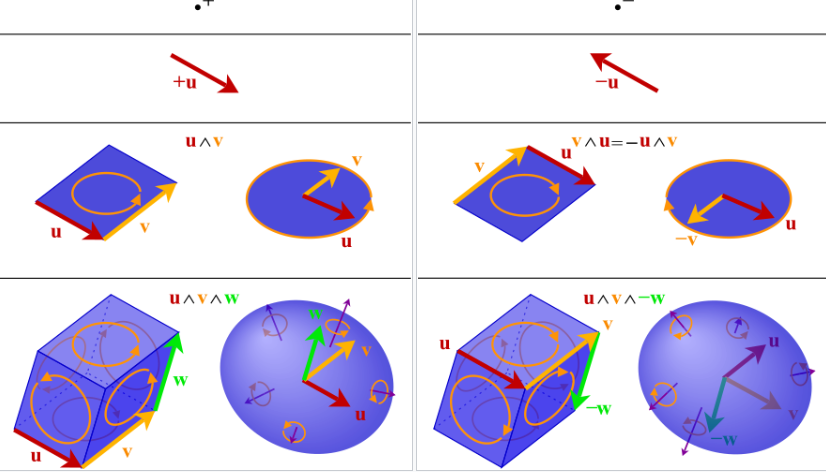
\includegraphics[scale =0.8]{wedge}
		\caption{Oriented $k$-volume of parallelopiped spanned by an ordered set of $k$-vectors. Changing the order corresponds to changing the orientation.}
	\end{center}
\end{figure}


\begin{theorem}[Universal property of exterior products]
	Let $V$ and $U$ be finite dimensional real vector spaces and denote by $\iota : V^k \to \bigwedge^k V$ the $k$-linear map $(v_1, \dots, v_k) \mapsto v_1 \wedge \dots \wedge v_k$. Then for every alternating $k$-linear map $\phi :V^k \to U$, there exists a unique linear map $\widetilde \phi : \bigwedge^k V \to U$ such that the diagram commutes
	\begin{center}
		\begin{tikzcd}
V^k \arrow[r, "\iota"] \arrow[rd, "\phi"'] & \bigwedge^k V \arrow[d, "\widetilde \phi"] \\
                                           & U                                         
\end{tikzcd}
	\end{center}
\end{theorem}

\begin{proof}
	By the universal property for tensor products, the $k$-linear map $\phi : V^k \to U$ descends uniquely to a linear map $\overline \phi : V^{\otimes k} \to U$ satisfying 
		\[ \overline \phi (v_1 \otimes \dots \otimes v_k) = \phi(v_1, \dots, v_k). \]
	We see from the alternating property of $\phi$ that $I \hookrightarrow  \ker \overline \phi$, so $\overline \phi$ descends to $\widetilde \phi : \bigwedge^k V \to U$ the unique linear map satisfying 
		\[ \widetilde \phi (v_1 \wedge \dots \wedge v_k) = \overline (v_1 \otimes \dots \otimes v_k) = \phi(v_1, \dots, v_k). \]
	The condition above can be rewritten as $\widetilde \phi \circ \iota = \phi$, completing the proof. 		
\end{proof}

\begin{corollary}
	If $V$ is a vector space of dimension $n$ and $\{e_1, \dots, e_n\}$ is a basis for $V$, then 
	\[ \{ e_{i_1} \wedge \dots \wedge e_{i_k} : i_1 < \dots, i_k \} \]
forms a basis for $\bigwedge^k V$, which therefore has dimension $\binom{n}{k}$ when $k \leq n$ and dimension zero when $k > n$.
\end{corollary}


\end{document}